\documentclass[border=2pt]{standalone}
\usepackage{tikz}
\usetikzlibrary{arrows.meta,chains,%
                    decorations.pathreplacing}
\usetikzlibrary{matrix,positioning,arrows.meta,arrows}
\usetikzlibrary{patterns}

\tikzset{
mymat/.style={
  matrix of nodes,
  nodes in empty cells,
  text height=2.5ex,
  text depth=0.75ex,
  text width=3.25ex,
  align=center,
  column sep=-\pgflinewidth
  }
}
\tikzset{
  rows/.style 2 args={
    sub@rows/.style={row ##1 column #2/.style={nodes={rectangle,draw=black}}},
    sub@rows/.list={#1}
  },
  box/.style 2 args={
    sub@box/.style={rows={#1}{##1}},
    sub@box/.list={#2}
  }
}
\pgfdeclarelayer{background}
\pgfdeclarelayer{foreground}
\pgfsetlayers{background,main,foreground}   %% some additional layers for demo


\begin{document}

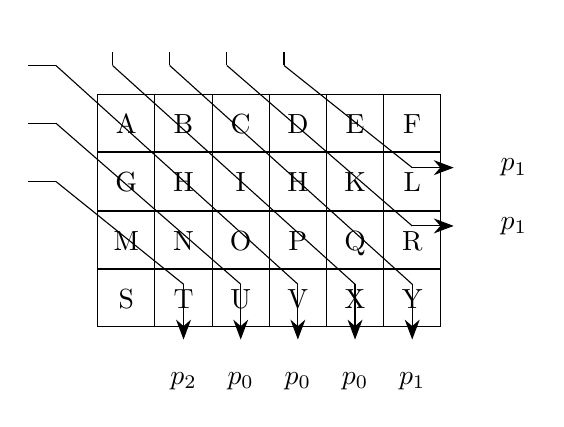
\begin{tikzpicture}[>=latex]
\matrix[mymat,anchor=west,
    box={2, 3, 4, 5}{2, 3, 4, 5, 6, 7}]
at (0,0) 
(mat1)
{ 
   &  &  &  &  &  &  & \\
   & A & B & C & D & E & F & \\
   & G & H & I & H & K & L & \\
   & M & N & O & P & Q & R & \\
   & S & T & U & V & X & Y & \\ };

\begin{scope}
\coordinate(bup) at([yshift=5pt]mat1-5-5.center);
\coordinate(bleft) at([xshift=-5pt]mat1-1-1.center);
\coordinate(bup-f) at([yshift=-15pt]mat1-5-5.center);
\coordinate(bleft-f) at([xshift=-15pt]mat1-1-1.center);

\draw (bup) -- (bleft);
\draw[-{Stealth[scale=1.5]}] (bup) -- (bup-f);
\draw (bleft) -- (bleft-f);
\node[below=of bup]{$p_0$};
\end{scope}

\begin{scope}
\coordinate(bup) at([yshift=5pt]mat1-5-4.center);
\coordinate(bleft) at([xshift=-5pt]mat1-2-1.center);
\coordinate(bup-f) at([yshift=-15pt]mat1-5-4.center);
\coordinate(bleft-f) at([xshift=-15pt]mat1-2-1.center);

\draw (bup) -- (bleft);
\draw[-{Stealth[scale=1.5]}] (bup) -- (bup-f);
\draw (bleft) -- (bleft-f);
\node[below=of bup]{$p_0$};
\end{scope}

\begin{scope}
\coordinate(bup) at([yshift=5pt]mat1-5-6.center);
\coordinate(bleft) at([xshift=-5pt]mat1-1-2.center);
\coordinate(bup-f) at([yshift=-15pt]mat1-5-6.center);
\coordinate(bleft-f) at([xshift=-5pt,yshift=5pt]mat1-1-2.center);

\draw (bup) -- (bleft);
\draw[-{Stealth[scale=1.5]}] (bup) -- (bup-f);
\draw (bleft) -- (bleft-f);
\node[below=of bup]{$p_0$};
\end{scope}

\begin{scope}
\coordinate(bup) at([yshift=5pt]mat1-5-7.center);
\coordinate(bleft) at([xshift=-5pt]mat1-1-3.center);
\coordinate(bup-f) at([yshift=-15pt]mat1-5-7.center);
\coordinate(bleft-f) at([xshift=-5pt,yshift=5pt]mat1-1-3.center);

\draw (bup) -- (bleft);
\draw[-{Stealth[scale=1.5]}] (bup) -- (bup-f);
\draw (bleft) -- (bleft-f);
\node[below=of bup]{$p_1$};
\end{scope}

\begin{scope}
\coordinate(bup) at([yshift=5pt]mat1-4-7.center);
\coordinate(bleft) at([xshift=-5pt]mat1-1-4.center);
\coordinate(bup-f) at([yshift=5pt,xshift=15pt]mat1-4-7.center);
\coordinate(bleft-f) at([xshift=-5pt,yshift=5pt]mat1-1-4.center);

\draw (bup) -- (bleft);
\draw[-{Stealth[scale=1.5]}] (bup) -- (bup-f);
\draw (bleft) -- (bleft-f);
\node[right=of bup]{$p_1$};
\end{scope}

\begin{scope}
\coordinate(bup) at([yshift=5pt]mat1-3-7.center);
\coordinate(bleft) at([xshift=-5pt]mat1-1-5.center);
\coordinate(bup-f) at([yshift=5pt,xshift=15pt]mat1-3-7.center);
\coordinate(bleft-f) at([xshift=-5pt,yshift=5pt]mat1-1-5.center);

\draw (bup) -- (bleft);
\draw[-{Stealth[scale=1.5]}] (bup) -- (bup-f);
\draw (bleft) -- (bleft-f);
\node[right=of bup]{$p_1$};
\end{scope}

\begin{scope}
\coordinate(bup) at([yshift=5pt]mat1-5-3.center);
\coordinate(bleft) at([xshift=-5pt]mat1-3-1.center);
\coordinate(bup-f) at([yshift=-15pt]mat1-5-3.center);
\coordinate(bleft-f) at([xshift=-15pt]mat1-3-1.center);

\draw (bup) -- (bleft);
\draw[-{Stealth[scale=1.5]}] (bup) -- (bup-f);
\draw (bleft) -- (bleft-f);
\node[below=of bup]{$p_2$};
\end{scope}

\end{tikzpicture}

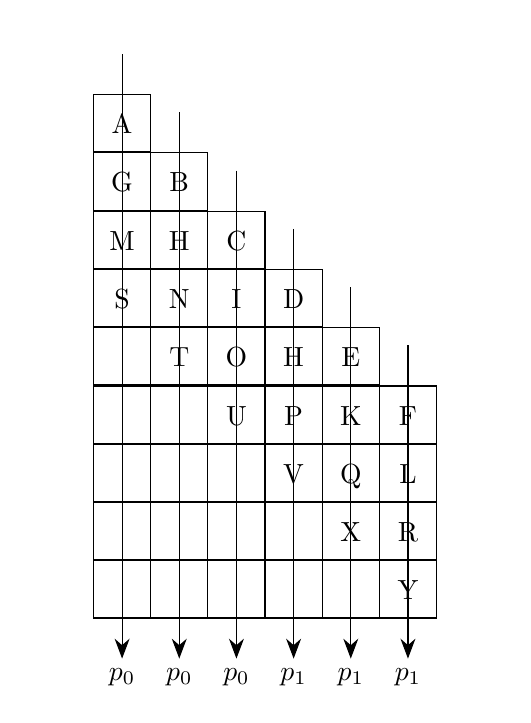
\begin{tikzpicture}[>=latex]
\matrix[mymat,anchor=west,
    box={2}{2},box={3}{2,3},box={4}{2,3,4},box={5}{2,3,4,5},
    box={6}{2,3,4,5,6},box={7}{2,3,4,5,6,7},box={8}{2,3,4,5,6,7},
    box={9}{2,3,4,5,6,7},box={10}{2,3,4,5,6,7}]
at (0,0) 
(mat1)
{ 
  &  &  &  &  &  &  & \\
  & A & \\
  & G & B & \\
  & M & H & C \\
  & S & N & I & D\\
  &   & T & O & H & E \\
  &   &   & U & P & K & F \\
  &   &   &   & V & Q & L \\
  &   &   &   &   & X & R \\
  &   &   &   &   &   & Y \\};


\begin{scope}
\coordinate(bup) at([yshift=25pt]mat1-2-2.center);
\coordinate(bleft) at([yshift=-25pt]mat1-10-2.center);

\draw[-{Stealth[scale=1.5]}] (bup) -- (bleft);
\node[below=-0pt of bleft]{$p_0$};
\end{scope}

\begin{scope}
\coordinate(bup) at([yshift=25pt]mat1-3-3.center);
\coordinate(bleft) at([yshift=-25pt]mat1-10-3.center);

\draw[-{Stealth[scale=1.5]}] (bup) -- (bleft);
\node[below=-0pt of bleft]{$p_0$};
\end{scope}

\begin{scope}
\coordinate(bup) at([yshift=25pt]mat1-4-4.center);
\coordinate(bleft) at([yshift=-25pt]mat1-10-4.center);

\draw[-{Stealth[scale=1.5]}] (bup) -- (bleft);
\node[below=-0pt of bleft]{$p_0$};
\end{scope}

\begin{scope}
\coordinate(bup) at([yshift=25pt]mat1-5-5.center);
\coordinate(bleft) at([yshift=-25pt]mat1-10-5.center);

\draw[-{Stealth[scale=1.5]}] (bup) -- (bleft);
\node[below=-0pt of bleft]{$p_1$};
\end{scope}

\begin{scope}
\coordinate(bup) at([yshift=25pt]mat1-6-6.center);
\coordinate(bleft) at([yshift=-25pt]mat1-10-6.center);

\draw[-{Stealth[scale=1.5]}] (bup) -- (bleft);
\node[below=-0pt of bleft]{$p_1$};
\end{scope}

\begin{scope}
\coordinate(bup) at([yshift=25pt]mat1-7-7.center);
\coordinate(bleft) at([yshift=-25pt]mat1-10-7.center);

\draw[-{Stealth[scale=1.5]}] (bup) -- (bleft);
\node[below=-0pt of bleft]{$p_1$};
\end{scope}

\end{tikzpicture}

\end{document}